\pdfbookmark{Общая характеристика работы}{characteristic}             % Закладка pdf
\section*{Общая характеристика работы}

\newcommand{\actuality}{\pdfbookmark[1]{Актуальность и степень разработанности темы исследования}{actuality}\textbf{\uline{Актуальность и степень разработанности темы исследования.}}}
\newcommand{\progress}{\pdfbookmark[1]{Разработанность темы}{progress}\underline{\textbf{\progressTXT}}}
\newcommand{\aim}{\pdfbookmark[1]{Цели}{aim}\underline{{\textbf\aimTXT}}}
\newcommand{\tasks}{\pdfbookmark[1]{Задачи}{tasks}\underline{\textbf{\tasksTXT}}}
\newcommand{\aimtasks}{\pdfbookmark[1]{Цели и задачи}{aimtasks}\aimtasksTXT}
\newcommand{\novelty}{\pdfbookmark[1]{Научная новизна}{novelty}\underline{\textbf{\noveltyTXT}}}
\newcommand{\influence}{\pdfbookmark[1]{Практическая значимость}{influence}\underline{\textbf{\influenceTXT}}}
\newcommand{\methods}{\pdfbookmark[1]{Методология и методы исследования}{methods}\underline{\textbf{\methodsTXT}}}
\newcommand{\defpositions}{\pdfbookmark[1]{Положения, выносимые на защиту}{defpositions}\underline{\textbf{\defpositionsTXT}}}
\newcommand{\reliability}{\pdfbookmark[1]{Достоверность}{reliability}\underline{\textbf{\reliabilityTXT}}}
\newcommand{\probation}{\pdfbookmark[1]{Апробация}{probation}\underline{\textbf{\probationTXT}}}
\newcommand{\contribution}{\pdfbookmark[1]{Личный вклад}{contribution}\underline{\textbf{\contributionTXT}}}
\newcommand{\publications}{\pdfbookmark[1]{Публикации}{publications}\underline{\textbf{\publicationsTXT}}}


{\actuality} <<Игровые>> взаимодействия, в которых каждый участник руководствуется принципами максимизации выигрыша в некоторой игре -- 
либо своего личного, либо целого коллектива («популяции») – существенно отличны от обычных физических взаимодействий. 
Дополненные механизмами обучения, оценки и адаптации, игровые взаимодействия определяют принципиально новый тип динамики или <<эволюции>> [1]. 
К настоящему времени стало понятно, что область применения игровой динамики гораздо шире социологии и экологии, и что соответствующие 
методы могут быть использованы для моделирования динамики финансовых рынков [2] и интерпретации процессов Бозе-Эйнштейн конденсации в открытых квантовых системах [3]. 

Объект исследования данной работы — процессы случайных блужданий, обусловленные конфликтным взаимодействием игроков. 
Модельный процесс представляет собой игру, в которой игроки управляют перемещением точки (индикатор положения) на квадратной решетке, 
делая независимый выбор одной из двух возможных стратегий (<<ход>>) на каждом шаге игры. Информация о возможных перемещениях точки 
(определяемых совместным выбором), открыта для обоих игроков и организована в виде матрицы. Целью первого игрока является максимально 
долгое удержание точки внутри ограниченной области, а второго -- максимально быстрое достижение ею поглощающей границы. 
Результатом игры («платежом») является время поглощения. 

Игры такого типа были определены в некоторых работах по теории игр и принятия решений еще в 1950-1960х годах [4,5]. 
Однако, в силу вычислительной сложности задачи, количественные результаты были получены только для очень простых моделей 
с тремя-пятью состояниями [6], что не позволяет делать заключения об асимптотических характеристиках процесса и использовать 
для их анализа статистический подход. Существует тесная связь между «играми на выживание» и процессами случайных блужданий, 
например, классическая задача о разорении игрока допускает прямую интерпретацию как процесс случайного блуждания на конечном интервале [6]. 

С другой стороны, проблема случайных блужданий в ограниченной области и такие вопросы, как оценка среднего времени достижения границы 
(или любого другого определённого региона). [7], в настоящее время испытывает очередную волну интереса, вызванную перспективами 
приложения этого подхода к проблемам молекулярной биологии, химической кинетики, и экологии [8-9]. 

Идея данной работы состоит в том, что игровые <<блуждания>> в конечных пространственных областях, ограниченных поглощающими границами 
(достижение границы является выигрышем одного из игроков и, соответственно, проигрышем его оппонента), 
могут быть исследованы и квантифицированы, используя методологию теории случайных блужданий. Более конкретно, 
предлагается исследовать распределение времени достижения границы (<<времени игры>>). Очевидно, что такое распределение 
будет существенно отличаться от распределения времени достижения границ для стандартных моделей случайных блужданий 
в той же ограниченной области [8]. Одна из задач -- построение стохастической модели, которая бы воспроизводила это распределение. 
В работе проводится сравнение теоретических результатов с экспериментальными данными, собранными c помощью мобильного приложения. 
Следует отметить, что использование методик таких экспериментов (в областях далеких от социологии, где, главным образом, эта методика локализована) 
является одним из новейших трендов в области прикладной математики и математического моделирования; см., например [10-12].
Данная работа предполагает проведение масштабного «полевого эксперимента» с участием реальных игроков. 
Таким образом, область исследований лежит на стыке трех областей: теории случайных блужданий, теории игр и принятия решений 
и технологии социальных экспериментов с использованием мобильных приложений. 

В соответствии с паспортом специальности 05.13.18 <<Математическое моделирование,
численные методы и комплексы программ>>, данная диссертация
относится к следующим областям исследований: <<3. Разработка, обоснование
и тестирование эффективных вычислительных методов с применением современных
компьютерных технологий>>, <<4. Реализация эффективных численных методов и алгоритмов в виде
комплексов проблемно-ориентированных программ для проведения
вычислительного эксперимента>> <<5. Комплексные исследования научных и
технических проблем с применением современной технологии математического
моделирования и вычислительного эксперимента>>, <<7. Разработка новых математических
методов и алгоритмов интерпретации натурного эксперимента на
основе его математической модели>>, <<8. Разработка систем компьютерного и имитационного моделирования>>.

\ifsynopsis
Этот абзац появляется только в~автореферате.
Для формирования блоков, которые будут обрабатываться только в~автореферате,
заведена проверка условия \verb!\!\verb!ifsynopsis!.
Значение условия задаётся в~основном файле документа (\verb!synopsis.tex! для
автореферата).
\else
Этот абзац появляется только в~диссертации.
Через проверку условия \verb!\!\verb!ifsynopsis!, задаваемого в~основном файле
документа (\verb!dissertation.tex! для диссертации), можно сделать новую
команду, обеспечивающую появление цитаты в~диссертации, но~не~в~автореферате.
\fi

% {\progress}
% Этот раздел должен быть отдельным структурным элементом по
% ГОСТ, но он, как правило, включается в описание актуальности
% темы. Нужен он отдельным структурынм элемементом или нет ---
% смотрите другие диссертации вашего совета, скорее всего не нужен.

{\aim} данной работы является получение информации о статистических
характеристиках процесса блужданий в ограниченной двухмерной области, индуцированного игровым
взаимодействием двух игроков-оппонентов и построение стохастической модели, способной воспроизвести эти характеристики. 

Для~достижения поставленной цели необходимо было решить следующие {\tasks} диссертационного исследования:
\begin{enumerate}[beginpenalty=10000] % https://tex.stackexchange.com/a/476052/104425
    \item Разработка стохастической модели блужданий на плоскости, управляемых
    игровым конфликтом, и получение характеристик игрового процесса.
    \item Разработка и имплементация алгоритмов для моделирования
    игровой пространственной динамики, используя стохастическую
    модель, получение информации о статистических характеристиках
    модельного процесса, таких как время достижения границы и его
    распределение.
    \item Реализация масштабной серии экспериментов с участием
    реальных игроков и получение статистически значимого массива
    данных.
    \item Исследование взаимосвязи результатов, полученных в ходе
    теоретического анализа, численного моделирования, и эксперимента, а
    также их совместная интерпретация.
\end{enumerate}


{\novelty}
В работе получены следующие новые научные результаты:
\begin{enumerate}[beginpenalty=10000] % https://tex.stackexchange.com/a/476052/104425
  \item Впервые предложен игровой конфликт двух игроков, управляющих блужданием фишки на плоскости, реализованный в виде мобильного приложения.
        Новизна подхода заключается в применении интернет-технологий для реализации игры одновременно учитывающей как 
        возможность создания игрового взаимодействия между игроками, так и процесса случайного блуждания.
  \item Впервые разработана стохастическая модель предложенной игровой динамики, позволяющая получить характеристики игрового процесса 
        и воспроизвести результаты масштабного эксперимента игр полученных реальными игроками. Новизна подхода состоит в возможности 
        исследования модельного процесса случайного блуждания, позволяющего воспроизвести экспериментально полученные характеристики,
        а также провести точное сравнение модели с полевым экспериментом.
  \item Разработаны и реализованы численные методы для расчета статистических характеристик игрового процесса при фиксированных заданных стратегиях игроков,
        таких как среднее время игры, распределение времен игры, распределение вероятностей наблюдения фишки в состояниях конечной решетки. 
  \item Выдвинута гипотеза об оптимальном среднем времени оптимальных стратегий для двух случаев игры против стратегии случайного равновероятного выбора, продемонстрирована
        оптимальность данных значений для малых размеров игрового поля и предложены классы стратегий, достигающие предполагаемой оптимальной оценки.
\end{enumerate}

%{\influence} \ldots

{\methods} 
В работе используются методы математического моделирования, теории игр, теории вероятностей, математической статистики, 
теории Марковских цепей, теории случайных блужданий, математического программирования, численного моделирования. 
Дополнительно используется подход к проведению масштабного полевого эксперимента с применением интернет-технологий и мобильных приложений.


{\defpositions}
\begin{enumerate}[beginpenalty=10000] % https://tex.stackexchange.com/a/476052/104425
  \item Построена стохастическая модель, описывающая игровой конфликт двух игроков, управляющих блужданием фишки на конечной квадратной решетке.
  \item Созданы методы для расчета статистических характеристик игрового процесса при фиксированных заданных стратегиях игроков,
        таких как среднее время игры, распределение времен игры, распределение вероятностей наблюдения фишки в состояниях конечной решетки. 
  \item Выдвинута гипотеза об оптимальном среднем времени для двух случаев игры против стратегии случайного равновероятного выбора,
        и установлена оптимальность данных значений для малых размеров игрового поля, а также найден класс стратегий, достигающих предполагаемой оптимальной оценки.
  \item Обнаружено соответствие эксперимента предложенной модели и установлены возникающие особенности синхронизации игроков, 
        а также выявлены отличия стратегий игроков от предполагаемых оптимальных стратегий
        на основе сравнения статистических свойств траекторий и стратегий участников масштабного эксперимента, 
        проведенного с применением мобильных и интернет-технологий.
  
\end{enumerate}

{\reliability} полученных результатов, научных положений и выводов,
полученных в диссертации, обеспечивается корректным обоснованием
постановок задач, точной формулировкой критериев, подтверждается результатами
вычислительных экспериментов по использованию предложенных в
диссертации методов и алгоритмов, сравнением полученных результатов с
проведёнными ранее исследованиями и перекрестной проверкой с применением трех различных методов.
Результаты находятся в соответствии с результатами, полученными другими авторами.

{\probation}
Основные результаты диссертационного исследования докладывались~на следующих научных конференциях и фестивалях:
\begin{itemize}
    \item XXVI научная конференция по радиофизике, посвященная 120-летию со дня рождения М.Т. Греховой. 2022, ННГУ им. Н.И. Лобачевского,
    Нижний Новгород.
    \item Всероссийский фестиваль молодежных инноваций Иннофест. 2020, ННГУ им. Н.И. Лобачевского,
    Нижний Новгород.
\end{itemize}


{\contribution} Решение задач диссертационного исследования, разработка стохастической модели, описывающей игровой конфликт двух игроков,
построение и реализация методов для расчета статистических характеристик, разработка гипотезы об оптимальном среднем времени игры
для двух случаев игры против стратегии случайного равновероятного выбора принадлежат автору лично.
Разработка мобильного приложения, разработка серверной части платформы, организация масштабного эксперимента 
и сопутствующих мероприятий выполнены при непосредственном активном участии автора.
Автор принимал прямое участие в постановке задач и анализе полученных результатов, а также в подготовке публикаций
в научных журналах и докладов на тематических конференциях.

\ifnumequal{\value{bibliosel}}{0}
{%%% Встроенная реализация с загрузкой файла через движок bibtex8. (При желании, внутри можно использовать обычные ссылки, наподобие `\cite{vakbib1,vakbib2}`).
    {\publications} Основные результаты по теме диссертации изложены
    в~2~печатных изданиях,
    0 из которых изданы в журналах, рекомендованных ВАК,
    1 "--- в тезисах докладов.
}%
{%%% Реализация пакетом biblatex через движок biber
    \begin{refsection}[bl-author, bl-registered]
        % Это refsection=1.
        % Процитированные здесь работы:
        %  * подсчитываются, для автоматического составления фразы "Основные результаты ..."
        %  * попадают в авторскую библиографию, при usefootcite==0 и стиле `\insertbiblioauthor` или `\insertbiblioauthorgrouped`
        %  * нумеруются там в зависимости от порядка команд `\printbibliography` в этом разделе.
        %  * при использовании `\insertbiblioauthorgrouped`, порядок команд `\printbibliography` в нём должен быть тем же (см. biblio/biblatex.tex)
        %
        % Невидимый библиографический список для подсчёта количества публикаций:
        \printbibliography[heading=nobibheading, section=1, env=countauthorvak,          keyword=biblioauthorvak]%
        \printbibliography[heading=nobibheading, section=1, env=countauthorwos,          keyword=biblioauthorwos]%
        \printbibliography[heading=nobibheading, section=1, env=countauthorscopus,       keyword=biblioauthorscopus]%
        \printbibliography[heading=nobibheading, section=1, env=countauthorconf,         keyword=biblioauthorconf]%
        \printbibliography[heading=nobibheading, section=1, env=countauthorother,        keyword=biblioauthorother]%
        \printbibliography[heading=nobibheading, section=1, env=countregistered,         keyword=biblioregistered]%
        \printbibliography[heading=nobibheading, section=1, env=countauthorpatent,       keyword=biblioauthorpatent]%
        \printbibliography[heading=nobibheading, section=1, env=countauthorprogram,      keyword=biblioauthorprogram]%
        \printbibliography[heading=nobibheading, section=1, env=countauthor,             keyword=biblioauthor]%
        \printbibliography[heading=nobibheading, section=1, env=countauthorvakscopuswos, filter=vakscopuswos]%
        \printbibliography[heading=nobibheading, section=1, env=countauthorscopuswos,    filter=scopuswos]%
        %
        \nocite{*}%
        %
        {\publications} Основные результаты по теме диссертации изложены в~\arabic{citeauthor}~печатных изданиях,
        \arabic{citeauthorvak} из которых изданы в журналах, рекомендованных ВАК\sloppy%
        \ifnum \value{citeauthorscopuswos}>0%
            , \arabic{citeauthorscopuswos} "--- в~периодических научных журналах, индексируемых Web of~Science и Scopus\sloppy%
        \fi%
        \ifnum \value{citeauthorconf}>0%
            , \arabic{citeauthorconf} "--- в~тезисах докладов.
        \else%
            .
        \fi%
        \ifnum \value{citeregistered}=1%
            \ifnum \value{citeauthorpatent}=1%
                Зарегистрирован \arabic{citeauthorpatent} патент.
            \fi%
            \ifnum \value{citeauthorprogram}=1%
                Зарегистрирована \arabic{citeauthorprogram} программа для ЭВМ.
            \fi%
        \fi%
        \ifnum \value{citeregistered}>1%
            Зарегистрированы\ %
            \ifnum \value{citeauthorpatent}>0%
            \formbytotal{citeauthorpatent}{патент}{}{а}{}\sloppy%
            \ifnum \value{citeauthorprogram}=0 . \else \ и~\fi%
            \fi%
            \ifnum \value{citeauthorprogram}>0%
            \formbytotal{citeauthorprogram}{программ}{а}{ы}{} для ЭВМ.
            \fi%
        \fi%
        % К публикациям, в которых излагаются основные научные результаты диссертации на соискание учёной
        % степени, в рецензируемых изданиях приравниваются патенты на изобретения, патенты (свидетельства) на
        % полезную модель, патенты на промышленный образец, патенты на селекционные достижения, свидетельства
        % на программу для электронных вычислительных машин, базу данных, топологию интегральных микросхем,
        % зарегистрированные в установленном порядке.(в ред. Постановления Правительства РФ от 21.04.2016 N 335)
    \end{refsection}%
    \begin{refsection}[bl-author, bl-registered]
        % Это refsection=2.
        % Процитированные здесь работы:
        %  * попадают в авторскую библиографию, при usefootcite==0 и стиле `\insertbiblioauthorimportant`.
        %  * ни на что не влияют в противном случае
        \nocite{vakbib2}%vak
        \nocite{patbib1}%patent
        \nocite{progbib1}%program
        \nocite{bib1}%other
        \nocite{confbib1}%conf
    \end{refsection}%
        %
        % Всё, что вне этих двух refsection, это refsection=0,
        %  * для диссертации - это нормальные ссылки, попадающие в обычную библиографию
        %  * для автореферата:
        %     * при usefootcite==0, ссылка корректно сработает только для источника из `external.bib`. Для своих работ --- напечатает "[0]" (и даже Warning не вылезет).
        %     * при usefootcite==1, ссылка сработает нормально. В авторской библиографии будут только процитированные в refsection=0 работы.
}

Результаты также направлены в 1 печатное издание в журнал Chaos (IF=3.741, Manuscript ID: CHA22-AR-00995), индексируемый
в Web of Science и Scopus, в котором получены положительные
рецензии, на данный момент вносятся коррективы в соответствии
с комментариями рецензетов. Также направлена заявка на регистрацию РИД
<<Программа для моделирования эволюции вероятности и 
расчета среднего времени поглощения в антагонистической игре двух игроков, управляющих 
случайным блужданием на решетке>>.

% При использовании пакета \verb!biblatex! будут подсчитаны все работы, добавленные
% в файл \verb!biblio/author.bib!. Для правильного подсчёта работ в~различных
% системах цитирования требуется использовать поля:
% \begin{itemize}
%         \item \texttt{authorvak} если публикация индексирована ВАК,
%         \item \texttt{authorscopus} если публикация индексирована Scopus,
%         \item \texttt{authorwos} если публикация индексирована Web of Science,
%         \item \texttt{authorconf} для докладов конференций,
%         \item \texttt{authorpatent} для патентов,
%         \item \texttt{authorprogram} для зарегистрированных программ для ЭВМ,
%         \item \texttt{authorother} для других публикаций.
% \end{itemize}
% Для подсчёта используются счётчики:
% \begin{itemize}
%         \item \texttt{citeauthorvak} для работ, индексируемых ВАК,
%         \item \texttt{citeauthorscopus} для работ, индексируемых Scopus,
%         \item \texttt{citeauthorwos} для работ, индексируемых Web of Science,
%         \item \texttt{citeauthorvakscopuswos} для работ, индексируемых одной из трёх баз,
%         \item \texttt{citeauthorscopuswos} для работ, индексируемых Scopus или Web of~Science,
%         \item \texttt{citeauthorconf} для докладов на конференциях,
%         \item \texttt{citeauthorother} для остальных работ,
%         \item \texttt{citeauthorpatent} для патентов,
%         \item \texttt{citeauthorprogram} для зарегистрированных программ для ЭВМ,
%         \item \texttt{citeauthor} для суммарного количества работ.
% \end{itemize}
% % Счётчик \texttt{citeexternal} используется для подсчёта процитированных публикаций;
% % \texttt{citeregistered} "--- для подсчёта суммарного количества патентов и программ для ЭВМ.

% Для добавления в список публикаций автора работ, которые не были процитированы в
% автореферате, требуется их~перечислить с использованием команды \verb!\nocite! в
% \verb!Synopsis/content.tex!. % Характеристика работы по структуре во введении и в автореферате не отличается (ГОСТ Р 7.0.11, пункты 5.3.1 и 9.2.1), потому её загружаем из одного и того же внешнего файла, предварительно задав форму выделения некоторым параметрам

%Диссертационная работа была выполнена при поддержке грантов \dots

%\underline{\textbf{Объем и структура работы.}} Диссертация состоит из~введения,
%четырех глав, заключения и~приложения. Полный объем диссертации
%\textbf{ХХХ}~страниц текста с~\textbf{ХХ}~рисунками и~5~таблицами. Список
%литературы содержит \textbf{ХХX}~наименование.

\pdfbookmark{Содержание работы}{description}                          % Закладка pdf
\section*{Содержание работы}
Во \underline{\textbf{введении}} обосновывается актуальность исследований, проводимых в рамках данной диссертационной работы, формулируется цель, ставятся задачи исследования, излагается научная новизна и практическая значимость представляемой работы, приводятся положения, выносимые на защиту. Введение содержит сведения о достоверности результатов и их апробации.

\underline{\textbf{Первая глава}} посвящена обзору научной литературы по различным видам таксиса, теории антагонистических игр, теории случайных блужданий, теории проведения социальных экспериментов с применением мобильных технологий.

В \underline{\textbf{разделе 1.1}} проводится обзор научной литературы, связанной с процессами движения у различных объектов живой природы и возникающими стратегиями поиска благоприятных условий, и рассмотрен один из наиболее изученных способов адаптации -- хемотаксис бактерий. 

Подвижность является важным фактором выживания видов, с помощью которого живые организмы адаптируются к условиям окружающей среды, получают питательные вещества, спасаются от токсинов и хищников и обмениваются генетической информацией посредством спаривания. Для описания движения организмов исследователи активно применяют концепцию случайных блужданий. Наиболее успешным при описании поведения движения различных простых организмов, таких как бактерии и насекомые, оказался способ описания, основанный на использовании в решении только локальной информации в пространстве и времени, доступной организму. Одна из наиболее известных стратегий движения -- <<run-and-tumble>> -- наблюдается у некоторых видов бактерий и других микроскопических агентов \cite{berg_coli_2004}. Стратегия состоит из чередующихся этапов <<run>> и <<tumble>>, соответствующих движению в фиксированном (или медленно меняющемся) направлении и повороту на одном месте на случайный угол. Длительность движения в фиксированном направлении аналогично является случайным процессом.

Адаптация бактерий к различным условиям окружающей среды возможна благодаря разнообразию размеров, форм, способов передвижения и способности к высокой чувствительности концентрации веществ. Отслеживание бактерией концентрации питательных веществ за счет механизма хемотаксиса приводит к движению в направлении аттрактанта или в направлении от различных вредоносных веществ -- репеллентов. Хотя паттерн движения бактерии остается неизменным, регуляция движения осуществляется за счет изменения длительностей движения бактерии на этапе <<run>>. Движение в сторону роста концентрации привлекающих веществ или в направлении убывания концентрации отталкивающих веществ приводит к увеличению длительности этапа <<run>> \cite{berg_chemotaxis_1972}.

Далее в \underline{\textbf{разделе 1.2}} проводится обзор научной литературы, демонстрирующей междисциплинарную природу возникновения процессов случайных блужданий. Приводятся такие работы, как задача Карла Пирсона, возникшая в биологии, но, как оказалось, уже решенная ранее Лордом Рэлеем при анализе колебаний в теории звука \cite{pearson_problem_1905,rayleigh_problem_1905}. Исследование свойств конфигураций гибких молекул в химии, описанное в работах Куна, привело к задаче свободно сочлененной цепи со звеньями фиксированной длины, но случайной ориентацией \cite{kuhn_uber_1930}. Возникшая задача представляла собой обобщение задачи Пирсона на трехмерный случай. В другой работе Н.~Темперлей заметил, что физические явления, связанные с решетками, могут быть решены в терминах случайных блужданий на решетках с ограничениями \cite{temperley_combinatorial_1956}.

Обнаружение случайных блужданий при рассмотрении модели ферромагнетизма на плоскости привело к появлению новой задачи анализа случайных блужданий без самопересечений \cite{gee_interaction_1946}. Один из важных классов случайных процессов был выделен Андреем Марковым \cite{markov_wahrscheinlichkeitsrechnung_1912}. Класс марковских процессов обладает характеристикой независимости будущих состояний от прошлых состояний при определенном настоящем состоянии. В конце раздела приводятся объекты, на которых можно осуществлять случайные блуждания.

Особыми случаями случайного блуждания являются полет Леви и модели диффузии, такие как броуновское движение. Впервые беспорядочное движение микроскопических видимых взвешенных частиц твердого вещества в жидкости или газе, вызываемое тепловым движением, наблюдал Роберт Браун в 1827 году при исследовании движения цветочной пыльцы в воде \cite{brown_brief_2015}. Начало строгого и количественного описания, связывающего микроскопическую и макроскопическую динамику частиц, положили работы Эйнштейна и Смолуховского, применивших вероятностно-статистический подход для описания эволюции плотности вероятности положения частиц \cite{einstein_uber_1905,vonsmoluchowski_zur_1906}.

Обнаружение процессов с аномальной диффузией, в которых нарушается классическое соотношение Эйнштейна, линейно связывающее средне-квадратичное отклонение положения блуждающей частицы и время, привело к развитию теории полетов Леви. Основной особенностью полетов Леви и модели диффузии является распространение частицы с бесконечной скоростью. Однако в реальных экспериментах максимальная скорость ограничена некоторой константной, что привело к разработке модели случайных блужданий Леви, учитывающих данную особенность \cite{gnedenko_predelnye_1949}.

Исследования в области движения живых организмов позволили обнаружить хорошее соответствие между подходом случайных блужданий Леви и экспериментальными данными \cite{shlesinger_levy_1986}. Стратегии движения, приводящие к распределениям Леви оказались более успешны для поиска пищи, чем броуновское движение. Дальнейший сбор сведений о разнообразных живых организмах показал, что многие из них имеют в своей основе движения механизм блужданий Леви.

В \underline{\textbf{разделе 1.3}} рассмотрены различные аспекты на стыке теории случайных блужданий и антагонистических игр. Теория игр тесно переплетается с проблемами случайных блужданий в широком спектре областей прикладных и фундаментальных исследований. Одним из примеров такой связи выступает задача о разорении игрока. Первые упоминания о задаче разорения игрока возникли в переписке Блеза Паскаля и Пьера Ферма в 1656 году при рассмотрении игры тремя костями между двумя игроками. Пьер де Каркави переформулировал задачу в письме Христиану Гюйгенсу и поставил вопрос о нахождении вероятности победы первого и второго игрока. Христиан Гюйгенс обновил формулировку задачи в своей работе и приблизил ее к классической: у игроков есть конечное количество монет, на каждом ходу подбрасывается ассиметричная монета, и выпадение аверса или реверса определяет какой игрок и кому отдает одну монету. Игрок, оставшийся без монет, считается проигравшим. В дополнении к вопросу о вероятностях выигрыша ставится вопрос нахождения среднего времени игры.

Поиск решений с использованием подхода теории случайных блужданий приводит к нахождению выражений в замкнутой форме для оценки как вероятности победы каждого из игроков, так и среднего количества ходов в игре в зависимости от начальных капиталов игроков. В предположении симметричности монеты и одинакового капитала игроков среднее время игры составляет $B^2$, где $B$ -- капитал каждого из игроков.

В продолжение анализа случайных блужданий рассматривается обобщение задачи о разорении игрока на большее количество измерений. Один из таких подходов обобщения был предложен израильскими математиками, рассматривавшими игру с учетом нескольких валют, имеющихся у игроков, при этом завершение игры определяется, когда у одного из игроков заканчиваются монеты любой из валют. Решение задачи о поиске среднего времени игры было найдено с применением дискретного преобразования Фурье и свойств спектра для матрицы Теплица. 

Естественным продолжением анализа является обобщение задачи о разорении игрока на случай произвольной многошаговой игры в условиях неопределенности. Работы Нэша о некооперативных играх с нулевой суммой предлагают общие свойства таких игр и наличие равновесия в стратегиях игроков \cite{nash_non-cooperative_1951}. Исследования Беллмана показали приблизительное решение для оптимальных стратегий игроков в произвольных многошаговых играх \cite{bellman_decision-making_1954}. В дальнейших работах Джон Милнор и Ллойд Шепли нашли точное решение игры \cite{milnor_games_1956}. Дополнительное обобщение игры было предложено И.\,В.~Романовским на случай влияния случайной компоненты на выигрыш игроков на каждом ходе \cite{romanovsky_1961}. 

Развитие сотовой связи и электроники позволило связать людей независимо от их георасположения, что привело к развитию области проведения социальных экспериментов с применением мобильных приложений и интернет-технологий. Анализ литературы продемонстрировал, что большая часть экспериментов, в которых применяются мобильные приложения, связана со здравоохранением. Однако применения были найдены и в других сферах, таких как экономика, мониторинг эффективности программ обучения, социальных явлениях и других. 

Сбор данных в таких экспериментах возможен как с датчиков устройства, так и информации о действиях пользователя в приложении, а также записей в дневнике о полученном опыте участника эксперимента. Дополнительная информация возникает при столкновении в игре человека с компьютерной системой или с другими игроками. Таким образом, применение мобильных приложений существенно расширило возможности по автоматическому и полуавтоматическому сбору данных и упростило методы проведения полевых экспериментов.

\underline{\textbf{Вторая глава}} посвящена моделированию процессов хемотаксиса бактерий, оценке средней скорости смещения бактерий для паттерна из двух чередующихся событий поворота, а также оценке параметров модели на основе численного эксперимента.

В \underline{\textbf{разделе 2.1}} предлагается математическая модель генерации степенных распределений, характеризующих время длительности движения бактерии в одном направлении, основанная на механизме дискретного шума \cite{bib1,confbib5}. Используя часть сигнальной сети хемотаксиса, определяющей химическую кинетику синтеза белка CheY-P, демонстрируется возможность возникновения переключений с промежуточной степенной статистикой в связи с генетическим шумом.

Переходы между различными значениями числа молекул белка CheY-P, обозначенного $Y$, в минимальной модели сигнального пути задаются следующим уравнением химической кинетики:
\begin{equation}
    \begin{aligned}
        Y \mathrel{\mathop{\rightleftarrows}^{\mathrm{K_{y}^{+}}}_{\mathrm{K_{y}^{-}}}} Y + 1,
    \label{eq:chem}
    \end{aligned}
\end{equation}
где $K_{y}^{+}=\frac{Y_0}{\tau}$, $K_{y}^{-}=\frac{Y+1}{\tau}$ -- коэффициенты интенсивностей перехода между состояниями, $Y_0$ -- равновесное число молекул, $\tau$ -- характерное время релаксации сигнального пути к равновесному числу молекул. Переходы между состояниями $X$ вращения моторов по часовой стрелке или против часовой стрелки можно представить в аналогичной форме. В разделе рассматриваются две формы коэффициентов: простая экспоненциальная форма и форма, учитывающая насыщение с ростом числа молекул, что является более биологически релевантным.

Численные результаты, представленные на Рисунке~\cref{fig:duration-pdf}, показывают, что коррелированный молекулярный шум дает степенное распределение длительностей, $p(t_{ccw}) \approx t^{-\gamma}$, в четко выраженном интервале (1.5-2 декады) с отсечкой при больших значениях длительности. При анализе второй формы коэффициентов демонстрируются схожие результаты. Дополнительно проводится систематическое исследование статистики в зависимости от значений параметров модели и демонстрируются области параметров, обладающие степенной асимптотикой с различным показателем $\gamma$.

\begin{figure}[ht]
    \centerfloat{
        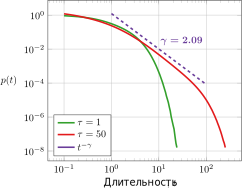
\includegraphics[scale=1]{genetic-noise/ru/fig1a}
    }
    \caption{
        Плотности вероятности длительностей в состоянии CCW для различных значений времени релаксации белка CheY-P, $\tau$. Остальные параметры: $\alpha = 10$, $Y_0 = 20$, $K_0 = 1$
    }
    \label{fig:duration-pdf}
\end{figure}

Применение подхода full-counting statistics позволяет независимо от природы основного кинетического уравнения оценить статистические свойства дискретной системы без применения ресурсоемкого алгоритма Гиллеспи \cite{gillespie_stochastic_2007}. Применение подхода основывается на представлении кинетики модели в виде марковской цепи с состоянием из пары $(X,Y)$, где $X$ -- направление вращения моторов, $Y$ -- количество белка. Тогда, за счет нахождения собственных чисел и векторов специальной матрицы переходов, стационарного распределения марковской цепи и применения формулы, полученной в настоящей диссертационной работе, можно вычислить плотность вероятности для распределения длительностей в каждом из двух состояний переменной $X$. 

В \underline{\textbf{разделе 2.2}} главы приводится обобщенная модель движения бактерий на случай двух чередующихся событий смены направления движения с различными углами поворота. 

Различные условия среды обитания и другие факторы эволюционно привели бактерии к необходимости разнообразия стратегий движения для ориентации в пространстве. Примером бактерии с характерно другим паттерном отличным от вида E.~coli служит вид V.~alginolyticus, обитающий в морской среде. Паттерн движения V.~alginolyticus состоит из трех этапов: прямолинейное движение, реверсивное движение и быстрый разворот. В этом паттерне бактерия движется некоторое время вперед, затем направление вращения моторов жгутиков меняется на противоположное и бактерия осуществляет реверсивное движение. 

В продолжение работы Йоханесса Тактикоса, в которой были найдены аналитические выражения для средней скорости смещения бактерий для частного случая паттерна с двумя углами (стратегия <<run-reverse-flick>>), в \underline{\textbf{разделе 2.3}} приводится решение задачи по нахождению формул для паттерна с произвольными средними косинусами углов поворота \cite{bib2}. Аналитическое исследование было проведено с применением теории линейного хемотаксиса. Предложенный метод легко обобщается на произвольную конечную цепочку событий поворота, имеющих различные характеристики, за счет решения системы линейных уравнений.

Итоговое выражение для средней скорости смещения при хемотаксисе бактерии с использованием паттерна с двумя поворотами записывается следующим образом:
\begin{equation}
    \begin{aligned}
        v_d=\frac{v_0^2\lambda_0^2W|\nabla c|\sum_{j=0}^{7} a_j(\alpha, \beta)D_r^{7-j}\lambda_0^j}{4\sum_{j=0}^{10}b_j(\alpha,\beta)D_r^{10-j}\lambda_0^j},
        \label{eq:drift-speed-solution}
    \end{aligned}
\end{equation}
где коэффициенты $a_j(\alpha,\beta), b_j(\alpha,\beta)$ определяются как полиномы от двух параметров, $W$ -- константа, характеризующая силу отклика бактерии, $|\nabla c|$ -- постоянный градиент концентрации химического вещества, $v_0$ -- постоянная скорость движения бактерии, $D_r$ -- коэффициент вращательной диффузии.

Полученная формула является обобщением частных случаев, которые были рассмотрены ранее в работах по исследованию хемотаксиса. Характерным способом движения для бактерии E.~coli является паттерн с одним углом поворота, рассмотренный в работе Яноша Локсей и соответствующий случаю $\alpha=\beta$ в формуле \cref{eq:drift-speed-solution}. Решение для случая двух углов с фиксированным вторым углом, равным $90^\circ$, полученное в работе Йоханнеса Тактикоса, также является частным случаем приведенной формулы.

Анализ выражения дает информацию о характерной зависимости $v_d$ от параметров: средняя скорость смещения обратно пропорциональна третьей степени коэффициента вращательной диффузии $D_r$, а также обратно пропорциональна базовой частоте переключения направления (соответственно прямо пропорционально средней длительности этапов направленного движения). 

В заключительном \underline{\textbf{разделе 2.3}} рассматривается разработанный алгоритм численного моделирования ансамбля бактерий в условиях как линейного, так и нелинейного градиента. Численные результаты согласуются с аналитически полученной средней скоростью смещения бактерий вдоль химического градиента \cite{confbib6}.



% картинку можно добавить так:
% \begin{figure}[ht]
%     \centerfloat{
%         \hfill
%         \subcaptionbox{\LaTeX}{%
%             \includegraphics[scale=0.27]{latex}}
%         \hfill
%         \subcaptionbox{Knuth}{%
%             \includegraphics[width=0.25\linewidth]{knuth1}}
%         \hfill
%     }
%     \caption{Подпись к картинке.}\label{fig:latex}
% \end{figure}

% Формулы в строку без номера добавляются так:
% \[
%     \lambda_{T_s} = K_x\frac{d{x}}{d{T_s}}, \qquad
%     \lambda_{q_s} = K_x\frac{d{x}}{d{q_s}},
% \]

\underline{\textbf{Третья глава}} описывает методы, подходы и алгоритмы, применяемые для анализа игрового процесса. В ходе описания приводится подробное построение стохастической модели игры и способы получения основных статистических свойств процесса. Далее демонстрируется способ построения различных оптимальных стратегий для нескольких случаев игры и нахождения оптимальных средних времен поглощения. В качестве подходов рассматриваются моделирование эволюции вероятности, расчет фундаментальной матрицы, численное моделирование методом Монте-Карло, численная оптимизация, теория рекурсивных игр и теория матричных игр. 

В \underline{\textbf{разделе 3.1}} предлагается новый игровой процесс между двумя игроками, управляющими на основе совместного выбора стохастическим движением фишки на дискретной решетке \cite{bib3}. Предложенная игра является частным случаем игр, рассматриваемых И.\,В.~Романовским, в которых учитывались свойство ограниченности пространства и случайная компонента в выборе игроков \cite{romanovsky_1961}. Игроки обладают противоположными целями по оптимизации времени игры, то есть числа ходов: первый игрок старается максимизировать время игры, тогда как второй -- минимизировать его. По достижении границы поля количество ходов, совершенных игроками, является временем игры и соответствует результату игры.

Модель игры представляет собой марковскую цепь с поглощающими состояниями, при этом вероятности перехода определяются совместным распределением стратегий двух игроков. Применяя теорию поглощающих Марковских цепей было получено решение задачи о вычислении среднего времени игры при заданных вероятностях выборов игроков для каждого состояния. 

Однако оценка распределения времен не была найдена в замкнутой форме. В связи с чем был предложен подход к моделированию эволюции вероятности найти фишку в некотором состоянии на решетке. С использованием модифицированной матрицы вероятностей переходов были получены оценки для распределения времен окончания игры, а также пространственные распределения на каждом шаге и свойства четности времени игры.

Дополнительным подходом, расширяющим информацию не только о статистических свойствах игры, но также и об индивидуальных траекториях, является численное моделирование. Применяя алгоритм Монте-Карло для симуляции траекторий, можно получить дополнительную информацию о структуре отдельных траекторий. Для визуализации были предложены различные способы, такие как визуализация всех ходов траектории на плоскости, визуализация ходов последовательными блоками и анимация движения фишки на поле. 

Хотя анализ теоретических аспектов игры возможен благодаря рассмотренным методам, выявление особенностей, возникающих при игре в Random Walk Game, требует проведения натурного эксперимента с участием реальных игроков. В \underline{\textbf{разделе 3.2.3}} описывается несколько различных организационных мероприятий, в рамках которых игрокам было предложено соревноваться друг с другом в игре. В результате было проведено около полутора тысяч матчей в течение 250 часов игр.

Проведение такого полномасштабного эксперимента стало возможно с использованием разработанного мобильного приложения, главный экран которого приведен на Рисунке~\cref{fig:screenshot_game_field_ref}, и применением подхода к автоматическому сбору данных о траекториях и выборах игроков в режиме онлайн посредством сети Интернет. Объединение игроков в мобильном приложении позволило привлечь участников по всему миру в условиях ограничений, связанных с пандемией, и успешно реализовать эксперимент. Для проектирования приложения был выбран подход MVVM, а для реализации приложения -- кроссплатформенная технология Xamarin на базе языка C$\mathsf{\#}$.

\begin{figure}[ht]
    \centerfloat{
        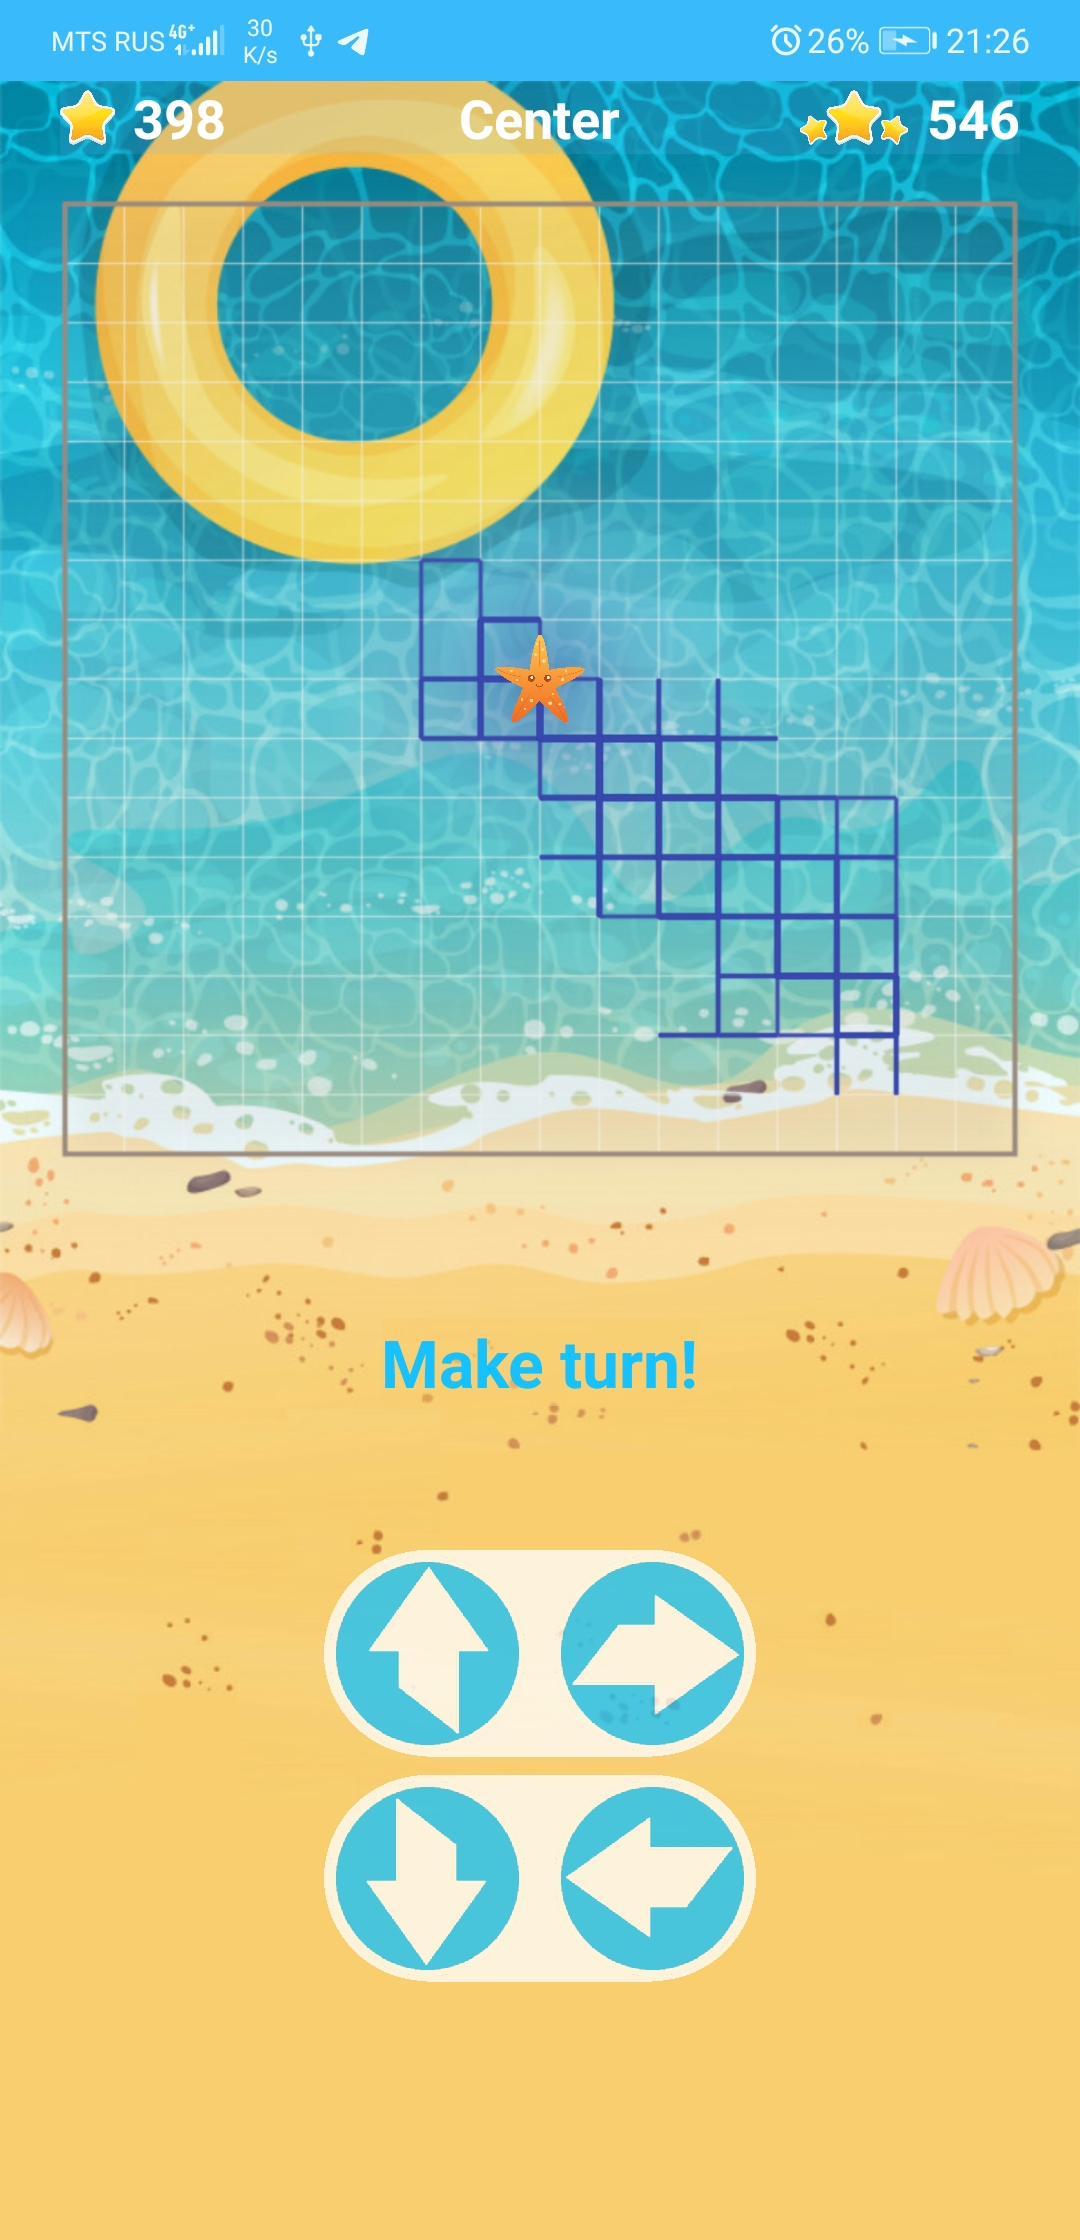
\includegraphics[scale=0.12]{screenshot_game_field}
    }
    \caption{
        Экран приложения Random Walk Game. Строка заголовка состоит из текущего количества ходов, 
        целей игроков и количества ходов в самой длинной игре. Игрок видит игровое поле, положение фишки и траекторию фишки. Внизу экрана показана управляющая матрица $2$ на $2$, которая определяет результат совместного выбора стратегий игроками A и B. Строки представляют собой возможный выбор стратегий для игрока A, а столбцы -- для игрока B. Результирующее направление движения  определяется стрелкой в ячейке, расположенной в соответствующих строке и столбце
    }\label{fig:screenshot_game_field_ref}
\end{figure}

Анализ и поиск оптимальных стратегий на основе предложенного представления в виде марковской цепи рассматривается в \underline{\textbf{разделе 3.3}}. Основная особенность рассматриваемой игры состоит в наличии случайной компоненты, не зависящей напрямую от игроков и лежащей в основе механики их взаимодействия. Для исключения влияния случайной компоненты на результирующий функционал был предложен подход к оценке среднего количества ходов в игре, что позволило найти оптимальные стратегии, дающие максимум или минимум среднего времени игры в зависимости от цели игрока.

Анализ игры осуществлен для различных случаев игрового взаимодействия: 
\begin{itemize}
    \item чистое случайное блуждание (выборы для обоих игроков равновероятно распределены и не зависят от положения фишки), в дальнейшем обозначается BvB -- Bot~versus~Bot;
    \item один игрок выбирает произвольную стратегию против стратегии равновероятного выбора, в дальнейшем обозначается PvE -- Player~versus~Environment, где Environment подразумевает внешнюю среду, не имеющую цель оптимизировать свою стратегию; дополнительно для различения цели игрока обозначим <<PvE A>> -- цель игрока оставаться как можно дольше внутри поля (игрок А), <<PvE B>> -- цель игрока как можно скорее достичь границу;
    \item оба игрока выбирают произвольную стратегию, в дальнейшем обозначается PvP -- Player~versus~Players.
\end{itemize}
Случай BvB вырождается в стандартную задачу случайного блуждания, на квадратной решетке, для которой ранее были получены результаты в виде двойной суммы оценки среднего времени игры. Случай PvE представляет собой задачу глобальной оптимизации с ограничениями, решение которой было найдено для размерностей поля $5$ и $7$ с применением техник символьных вычислений в математическом пакете Wolfram Mathematica. 

Значения среднего времени игры для малых размеров поля и особенности полученных стратегий привели к появлению гипотезы об оптимальном среднем времени игры для случая PvE. С использованием сведения задачи к одномерной Марковской цепи была показана достижимость предполагаемых оптимальных средних времен, которые при игре за центр представляются в виде: $\boldsymbol{\mathsf{t_n^{PvE A}}} = (n-2)^2$, а в случае игры за границу в виде: $\boldsymbol{\mathsf{t_n^{PvE B}}} = \frac{(n-1)^2}{4}$. Предложены различные стратегии, позволяющие достичь данных оценок \cite{confbib1}. Найденные оценки зависимости среднего времени игры от размера поля для трех случаев представляют собой квадратичную функцию с различными коэффициентами.

Случай PvP, в котором игроки оптимизируют свои стратегии, представляет собой задачу поиска максимина и минимакса функционала среднего времени игры, зависящего от набора частот, выбираемых игроками для каждого узла решетки. В такой постановке задача становится трудно разрешимой с применением методов численной оптимизации и требует применения других подходов. Решением задачи выступает сведение предложенной игры к рекурсивному представлению цепочки из матричных игр $2 \times 2$. Тогда нахождение оптимальных стратегий сводится к поиску неподвижной точки отображения цен. Применение данного подхода привело к получению оптимальных средних времен игры и оптимальных стратегий в случае PvP, а также позволило подтвердить гипотезу об оптимальных стратегиях для случаев PvE.

В \underline{\textbf{разделе 3.4}} описываются результаты численного анализа времен игры для трех случаев игры с применением различных численных подходов, рассмотренных в разделе 3.2, а также проводится анализ стратегий игроков и статистических свойств распределений для полученных экспериментальных игр. 

Сравнение результатов модели и эксперимента показывает высокую точность соответствия среднего времени игры между ними для всех случаев игры. Однако при рассмотрении случая игры двух игроков были обнаружены сверхдлинные игры, наличие которых было крайне маловероятно, учитывая найденное распределение времен игры при общей стратегии всех участников. Анализ таких игр показал отклонение статистики среднего времени игры от модели столкновения индивидуальных стратегий. Такое несоответствие связано с отсутствием свойства марковости процесса игры в этих отдельных случаях, что, в свою очередь, может быть связано с возникновением <<синхронизации>> принятия решений игроками в условиях накопленной усталости.

Экспериментальные значения среднего времени игры для случая PvP, представленные на Рисунке~\cref{fig:mean-times}, оказались близки к оптимальным значениям в игре, что подтверждает высокую предсказательную силу предложенной модели при реальной игре. Несмотря на это, в случаях игры против стратегии случайного равновероятного выбора игроки нарушали правила оптимальных стратегий, рассмотренные в настоящей диссертационной работе, что приводило к ухудшению значений среднего времени игры \cite{confbib4}. В случае игры за границу для оптимальной игры необходимо выбирать одномерный отрезок состояний, однако участники игры старались найти стратегию не только на прямой, но и на всем поле целиком. Игра за центр против стратегии случайного равновероятного выбора для оптимальной стратегии требует соблюдения единственного условия -- игра завершается только в углах на главной диагонали решетки. Нарушение этого правила значительно уменьшает вероятность остаться внутри поля. 

\begin{figure}[ht]
    \centerfloat{
        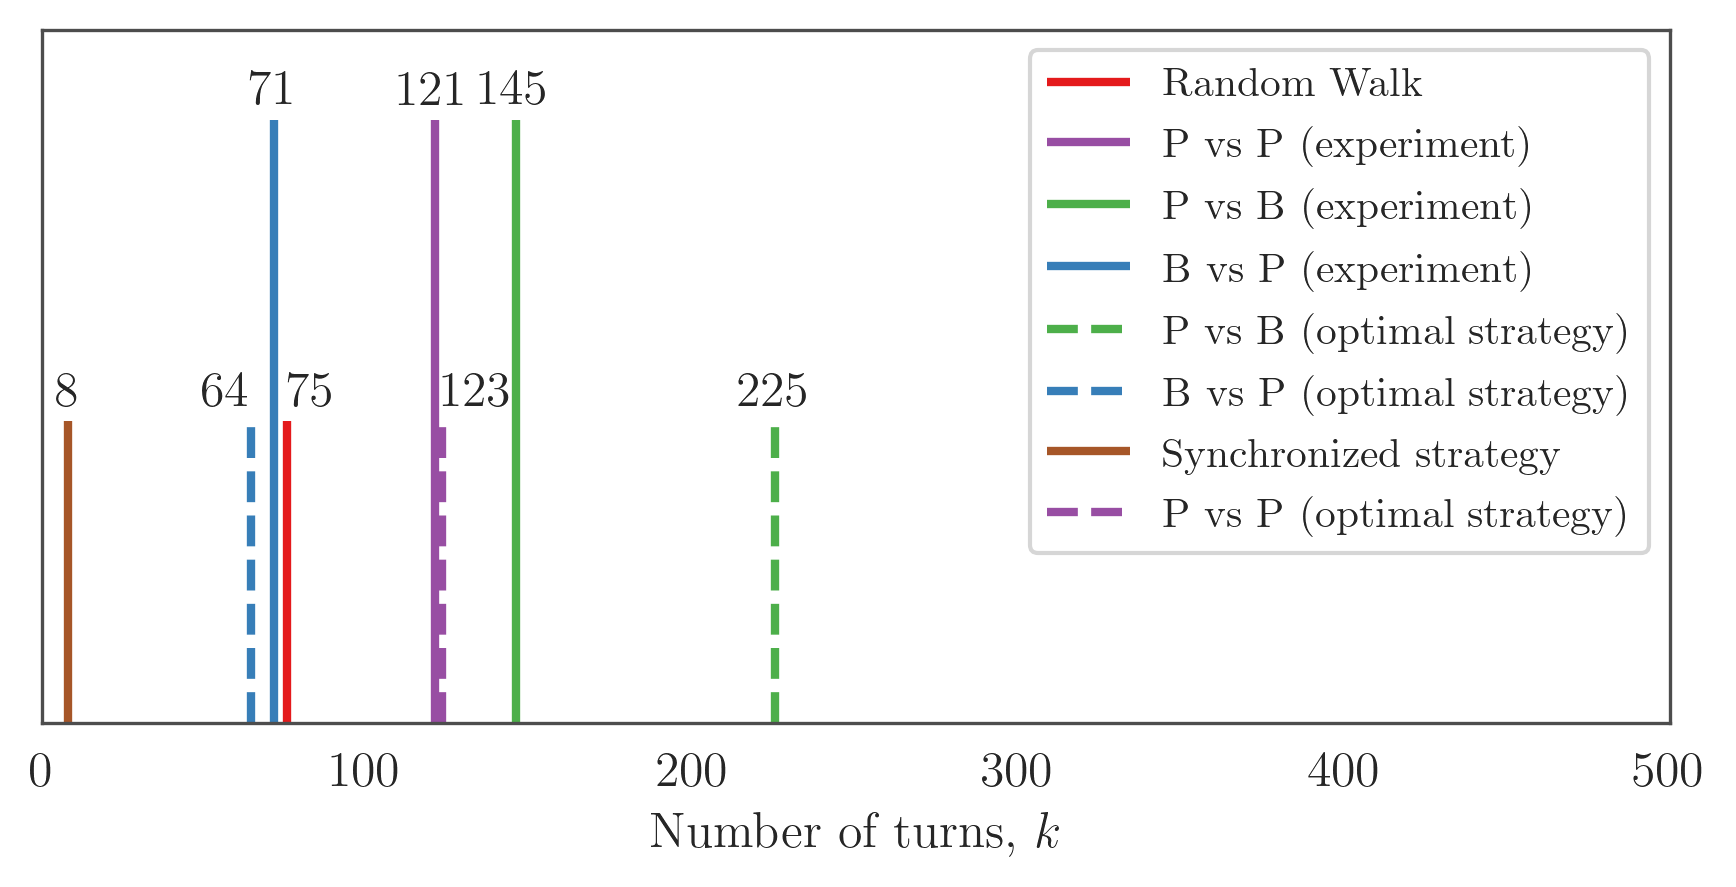
\includegraphics[width=\textwidth,keepaspectratio,clip]{rw-game/ru/fig2p_v3.png}
    }
    \caption{
        Среднее время игры, полученное в эксперименте, в сравнении с различными стратегиями и чистым случайным блужданием
    }  
    \label{fig:mean-times}
\end{figure}

Дальнейший анализ проводился для четности времени игры, в котором была выявлена неравномерность вероятности закончить игру на четном и нечетном ходе. При этом соотношение между этими двумя величинами различается в зависимости от случая игры. 

В заключительных подразделах главы были проведены исследование распределения вероятности обнаружения фишки в некотором состоянии и анализ обобщенных стратегий группы участников эксперимента. Была показана схожесть паттернов стратегий игроков с оптимальными стратегиями для всех случаев игры.

В ходе проведения анализа игровой динамики был разработан программный комплекс и получено свидетельство о государственной регистрации программы для ЭВМ для моделирования игровой динамики \cite{progbib1}.

\underline{\textbf{Раздел 3.5}} посвящен аспекту игрового процесса, связанному с когнитивной составляющей игроков. Важным фактором, влияющим на способность принимать решения, являются возрастные изменения мозга человека. На основе трех выбранных когнитивных тестов была разработана модель машинного обучения оценки когнитивного возраста индивидуума со средней абсолютной ошибкой 8.62 года \cite{bib4}. Основные показатели, оцениваемые предложенными тестами, включают сенсомоторную реакцию, определяющую степень сохранности участков мозга и избирательное внимание, а также способность к цветовому различению, отражающую информацию об уровне рабочей памяти и внимания, а также об эмоциональном напряжении участников \cite{confbib2}. Дополнительно была обнаружена более высокая корреляционная связь когнитивных показателей с биологическим возрастом индивидуума, чем с его хронологическим возрастом \cite{confbib3}. В результате был разработан программный комплекс и получено свидетельство о государственной регистрации программы для ЭВМ для оценки когнитивного возраста индивидуума \cite{progbib2}.

% Можно сослаться на свои работы в автореферате. Для этого в файле
% \verb!Synopsis/setup.tex! необходимо присвоить положительное значение
% счётчику \verb!\setcounter{usefootcite}{1}!. В таком случае ссылки на
% работы других авторов будут подстрочными.
% Изложенные в третьей главе результаты опубликованы в~\cite{vakbib1, vakbib2}.
% Использование подстрочных ссылок внутри таблиц может вызывать проблемы.

\FloatBarrier
\pdfbookmark{Заключение}{conclusion}                                  % Закладка pdf
В \underline{\textbf{заключении}} приведены основные результаты работы, которые заключаются в следующем:
%% Согласно ГОСТ Р 7.0.11-2011:
%% 5.3.3 В заключении диссертации излагают итоги выполненного исследования, рекомендации, перспективы дальнейшей разработки темы.
%% 9.2.3 В заключении автореферата диссертации излагают итоги данного исследования, рекомендации и перспективы дальнейшей разработки темы.
\begin{enumerate}
  \item Построена стохастическая модель генерации степенных распределений длительностей нахождения системы в одном из двух состояний за счет дробового шума. Получен способ оценки распределения длительностей для модели. Найдены параметры для генерации двух чередующихся режимов: степенное распределение и экспоненциальное распределение длительностей.
  \item Получена аналитическая форма средней скорости колонии бактерий в случае паттерна движения с двумя чередующимися углами. Проведенный численный эксперимент позволил подтвердить корректность формулы при малом химическом градиенте, а также продемонстрировать наличие отклонений при большом градиенте. 
  \item Получена оценка параметров химической чувствительности бактерий и коэффициента диффузии при их движении в условиях нелинейной радиальной концентрации химического вещества с применением численного эксперимента.
  \item Построена стохастическая модель, описывающая предложенный игровой конфликт двух игроков, управляющих блужданием фишки на конечной квадратной решетке. 
  \item Разработаны методы для расчета статистических характеристик игрового процесса при фиксированных заданных стратегиях игроков, таких как среднее время игры, распределение времен игры, распределение вероятностей наблюдения фишки в состояниях конечной решетки. 
  \item Вычислены оптимальные средние времена для трех случаев игры, предложены классы оптимальных стратегий и визуализированы конкретные стратегии. Предложен подход для нахождения оптимальных стратегий при произвольной стратегии оппонента, а также при оптимальной стратегии.
  \item Разработано мобильное приложение Random Walk Game, реализующее игровую механику посредством сети интернет с использованием созданного веб-сервера по обработке и хранению результатов игр участников. Дополнительно разработан веб-сайт для отображения статистической информации по результатам игр участников в режиме реального времени. Приложение опубликовано в открытом доступе на двух маркетплейсах для платформ Android и iOS.
  \item Проведен масштабный эксперимент с применением мобильных и интернет-технологий, привлекший более 100 участников и позволивший собрать более 1500 игр Random Walk Game. 
  \item Подтверждено соответствие эксперимента предложенной модели для трех случаев игры на основе сравнения распределений и соответствующих средних времен игры. 
  \item Установлены возникающие особенности синхронизации игроков при длительных играх, связанные со снижением концентрации игроков. Длительные игры утомляют игроков, что снижает способность человека генерировать чисто случайную последовательность выборов.
  \item Выявлены отличия стратегий игроков от оптимальных стратегий на основе сравнения статистических свойств траекторий и стратегий участников для случаев игры против стратегии равновероятного случайного выбора.
\end{enumerate}


\pdfbookmark{Литература}{bibliography}                                % Закладка pdf
% При использовании пакета \verb!biblatex! список публикаций автора по теме
% диссертации формируется в разделе <<\publications>>\ файла
% \verb!common/characteristic.tex!  при помощи команды \verb!\nocite!

\ifdefmacro{\microtypesetup}{\microtypesetup{protrusion=false}}{} % не рекомендуется применять пакет микротипографики к автоматически генерируемому списку литературы
\urlstyle{rm}                               % ссылки URL обычным шрифтом
\ifnumequal{\value{bibliosel}}{0}{% Встроенная реализация с загрузкой файла через движок bibtex8
    \renewcommand{\bibname}{\large \bibtitleauthor}
    \nocite{*}
    \insertbiblioauthor           % Подключаем Bib-базы
    %\insertbiblioexternal   % !!! bibtex не умеет работать с несколькими библиографиями !!!
}{% Реализация пакетом biblatex через движок biber
    % Цитирования.
    %  * Порядок перечисления определяет порядок в библиографии (только внутри подраздела, если `\insertbiblioauthorgrouped`).
    %  * Если не соблюдать порядок "как для \printbibliography", нумерация в `\insertbiblioauthor` будет кривой.
    %  * Если цитировать каждый источник отдельной командой --- найти некоторые ошибки будет проще.
    %
    %% authorvak
    %\nocite{vakbib1}%
    %\nocite{vakbib2}%
    %
    %% authorwos
    %\nocite{wosbib1}%
    %
    %% authorscopus
    %\nocite{scbib1}%
    %
    %% authorpathent
    %\nocite{patbib1}%
    %
    %% authorprogram
    %\nocite{progbib1}%
    %
    %% authorconf
    \nocite{confbib1}%
    %\nocite{confbib2}%
    %
    %% authorother
    \nocite{bib1}%
    \nocite{bib2}%

    \ifnumgreater{\value{usefootcite}}{0}{
        \begin{refcontext}[labelprefix={}]
            \ifnum \value{bibgrouped}>0
                \insertbiblioauthorgrouped    % Вывод всех работ автора, сгруппированных по источникам
            \else
                \insertbiblioauthor      % Вывод всех работ автора
            \fi
        \end{refcontext}
    }{
        \ifnum \totvalue{citeexternal}>0
            \begin{refcontext}[labelprefix=A]
                \ifnum \value{bibgrouped}>0
                    \insertbiblioauthorgrouped    % Вывод всех работ автора, сгруппированных по источникам
                \else
                    \insertbiblioauthor      % Вывод всех работ автора
                \fi
            \end{refcontext}
        \else
            \ifnum \value{bibgrouped}>0
                \insertbiblioauthorgrouped    % Вывод всех работ автора, сгруппированных по источникам
            \else
                \insertbiblioauthor      % Вывод всех работ автора
            \fi
        \fi
        %  \insertbiblioauthorimportant  % Вывод наиболее значимых работ автора (определяется в файле characteristic во второй section)
        \begin{refcontext}[labelprefix={}]
            \insertbiblioexternal            % Вывод списка литературы, на которую ссылались в тексте автореферата
        \end{refcontext}
        % Невидимый библиографический список для подсчёта количества внешних публикаций
        % Используется, чтобы убрать приставку "А" у работ автора, если в автореферате нет
        % цитирований внешних источников.
        \printbibliography[heading=nobibheading, section=0, env=countexternal, keyword=biblioexternal, resetnumbers=true]%
    }
}
\ifdefmacro{\microtypesetup}{\microtypesetup{protrusion=true}}{}
\urlstyle{tt}                               % возвращаем установки шрифта ссылок URL
